\section{eo\-EPReduce$<$ EOT $>$ Class Template Reference}
\label{classeo_e_p_reduce}\index{eoEPReduce@{eoEPReduce}}
EP truncation method (some global stochastic tournament + sort) Softer selective pressure than pure truncate.  


{\tt \#include $<$eo\-Reduce.h$>$}

Inheritance diagram for eo\-EPReduce$<$ EOT $>$::\begin{figure}[H]
\begin{center}
\leavevmode
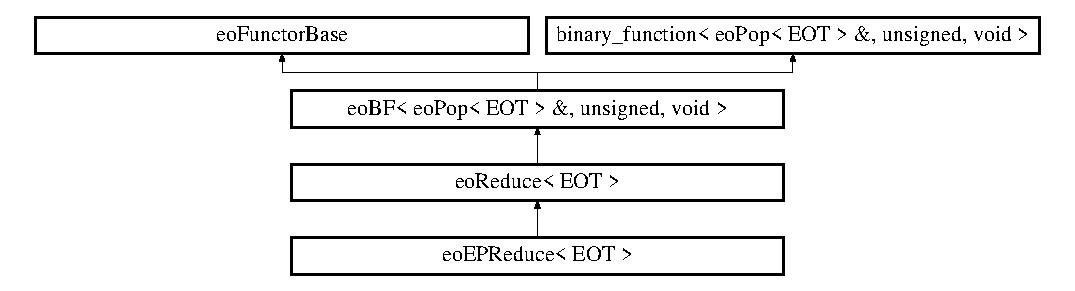
\includegraphics[height=3.45679cm]{classeo_e_p_reduce}
\end{center}
\end{figure}
\subsection*{Public Types}
\begin{CompactItemize}
\item 
typedef EOT::Fitness {\bf Fitness}\label{classeo_e_p_reduce_w0}

\item 
typedef std::pair$<$ float, typename {\bf eo\-Pop}$<$ {\bf EOT} $>$::iterator $>$ {\bf EPpair}\label{classeo_e_p_reduce_w1}

\begin{CompactList}\small\item\em helper struct for comparing on std::pairs \item\end{CompactList}\end{CompactItemize}
\subsection*{Public Member Functions}
\begin{CompactItemize}
\item 
{\bf eo\-EPReduce} (unsigned \_\-t\_\-size)\label{classeo_e_p_reduce_a0}

\item 
void {\bf operator()} ({\bf eo\-Pop}$<$ {\bf EOT} $>$ \&\_\-newgen, unsigned \_\-newsize)\label{classeo_e_p_reduce_a1}

\begin{CompactList}\small\item\em The pure virtual function that needs to be implemented by the subclass. \item\end{CompactList}\end{CompactItemize}
\subsection*{Private Attributes}
\begin{CompactItemize}
\item 
unsigned {\bf t\_\-size}\label{classeo_e_p_reduce_r0}

\end{CompactItemize}


\subsection{Detailed Description}
\subsubsection*{template$<$class EOT$>$ class eo\-EPReduce$<$ EOT $>$}

EP truncation method (some global stochastic tournament + sort) Softer selective pressure than pure truncate. 



Definition at line 83 of file eo\-Reduce.h.

The documentation for this class was generated from the following file:\begin{CompactItemize}
\item 
eo\-Reduce.h\end{CompactItemize}
